% 
% Lecture Template for ME3050 -  Dynamics Modeling and Controls - Tennessee Technological University
%
% Spring 2020 - Summer 2020
% Tristan Hill, May 07, 2020
% Dyanmics Review - Topic 6 - Particles and Bodies
%

\documentclass{beamer}                         % for presentation (has nav buttons at bottom)
%\documentclass[handout]{beamer}  % for handout 
\usepackage{beamerthemesplit}
\usepackage{amsmath}
\usepackage{listings}
\usepackage{multicol}
\usepackage{framed}

\beamertemplateballitem

\definecolor{TTUpurple}{rgb}{0.3098, 0.1607, 0.5176} % TTU Purple (primary)
\definecolor{TTUgold}{rgb}{1.0000, 0.8666, 0.0000} % TTU Gold (primary)

\setbeamercolor{palette primary}{bg=TTUpurple,fg=TTUgold}
\setbeamercolor{palette secondary}{bg=black,fg=TTUgold}
\setbeamercolor{palette tertiary}{bg=black,fg=TTUpurple}
\setbeamercolor{palette quaternary}{bg=TTUgold,fg=black}
\setbeamercolor{structure}{fg=TTUpurple} % itemize, enumerate, etc
\setbeamercolor{section in toc}{fg=TTUpurple} % TOC sections

%\usefonttheme{professionalfonts}

\newcommand{\Lagr}{\mathcal{L}} % lagrangian

\newcommand{\vspccc}{\vspace{6mm}\\} % large vertical space
\newcommand{\vspcc}{\vspace{4mm}\\}   % medium vertical space
\newcommand{\vspc}{\vspace{2mm}\\}     % small vertical space

\newcommand{\hspcccc}{\hspace{10mm}} % large horizontal space
\newcommand{\hspccc}{\hspace{6mm}} % large horizontal space
\newcommand{\hspcc}{\hspace{4mm}}   % medium horizontal space
\newcommand{\hspc}{\hspace{2mm}}     % small horizontal space


\author{ME3050 - Dynamics Modeling and Controls}%\\Tennessee Technological University \\} % original formatting from Mike Renfro, September 21, 2004

\newcommand{\MNUM}{2\hspace{2mm}} % Module number
\newcommand{\TNUM}{6\hspace{2mm}} % Topic number 
\newcommand{\moduletitle}{Dynamics Review }
\newcommand{\topictitle}{Particles and Bodies } 

\title{Module \MNUM - \moduletitle}

\date{May 29, 2020}

\begin{document}

\lstset{language=MATLAB,basicstyle=\ttfamily\small,showstringspaces=false}

\frame{\titlepage \center\begin{framed}\Large \textbf{Topic \TNUM - \topictitle}\end{framed} \vspace{5mm}}

% Section 0: Outline

\frame{

\large \textbf{Topic \TNUM - \topictitle} \vspace{3mm}\\

\begin{itemize}
	\item Particle Motion\vspace{3mm}\\ % Section 1
	\item Rigid Body Motion\vspace{3mm}\\% Section 2
	\item Is rigid body motion realistic?\vspace{3mm}\\ %Section 3
	\item Motion in ME3050\vspace{3mm}\\ % Section 4
\end{itemize}
}

% Section 1: 
\section{Particle Motion}

\frame{
\frametitle{Particle Motion}

In your dynamics course you derived and used these equations. \vspcc

			\scalebox{1.5}{$\vec{v}(t)=\frac{d\vec{r}}{dt}=v\hat{e_t}$}  \vspc

			\scalebox{1.5}{$\vec{a}(t)=\frac{d\vec{v}}{dt}=\dot{v}\hat{e_t}+\vec{v}\frac{ds}{dt}\frac{d\hat{e_t}}{ds}=\dot{v}\hat{e_t}+\frac{\nu^2}{\rho}\hat{e_n}$}  \vspc
		
			\scalebox{1.5}{$\frac{d\hat{e_t}}{ds}=\kappa \hat{e_n} $}\vspcc

Do you remeber these? Do they make sense to you?

}

% Section 2: 
\section{Rigid Body Motion}

\frame{
\frametitle{Rigid Body Motion}

\scalebox{1.25}{$\frac{d}{dt}|r_{pq}|^2=\frac{d}{dt}(\vec{r}_{pq}\cdotp\vec{r}_{pq})=2\vec{r}_{pq}\cdotp\frac{d\vec{r}_{pq}}{dt}=0$} \vspccc

In a rigid body motion, the body remains rigid and does not deform. This is intuitive but In mechanics a different definition is used. \vspc
%{\bf Mathematical Definition:}

In a rigid body motion all points on a single body rotate about a common point in space at the same anguar velocity. This point is known as the instantaneous center of rotation (ICR).
	
}

% Section 3: 
\section{Is rigid body motion realistic?}
\frame{

\frametitle{Is rigid body motion realistic?}

Consider a typical hobbyist quadcopter. Is the frame rigid?  \vspc

Is flight a rigid body motion?  \vspcc

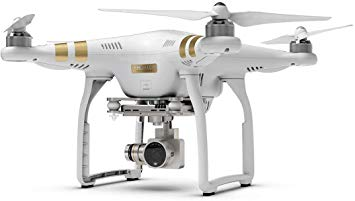
\includegraphics[scale=0.35]{dji_phantom.jpg} 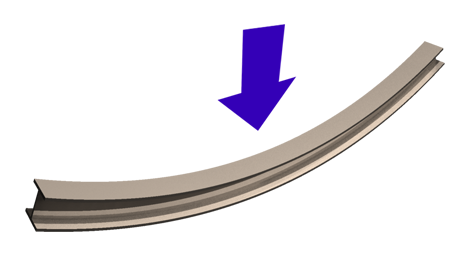
\includegraphics[scale=0.20]{beam_bending_01.png}\hspccc \scalebox{6}{?} 

}

\frame{
\frametitle{Example of Non-Rigid Body Motion or System}

\begin{multicols}{2}
 Traditionally engineers build machines that are strong and stiff. Name one machine that must be as strong and stiff as possible. \vspcc

 Can you think of a machine or system that relies on a non-rigid body motion or system?
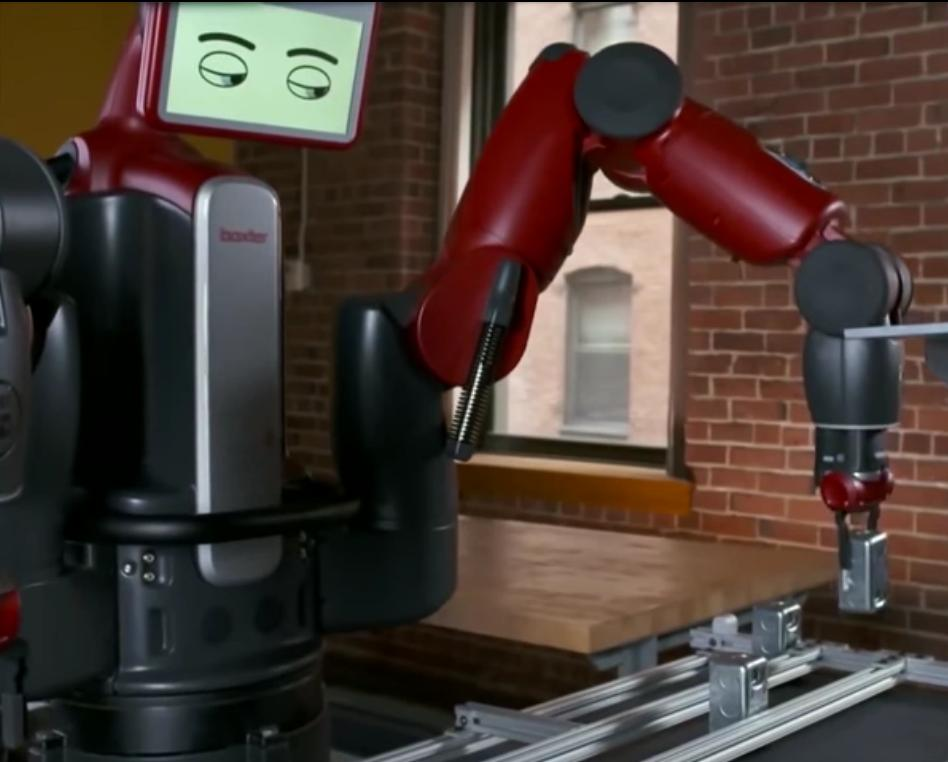
\includegraphics[scale=.20]{baxter_fig1.jpg}
\end{multicols}

}

% Section 4: 
\section{Motion in ME3050}

\frame{
\frametitle{Motion in ME3050}

In DMC we will study systems that undergo simple motions. \vspc
 
Therefore, we will focus on the system dynamics of translational and rotational engineering problems in which the motion is contrained to straightline or circlar paths. 

}






%	\item \textbf{ \LARGE \B Dynamic\K} \\
%			
%			\Large{"Dynamics is the study of how moving objects behave. Dynamics is the part of mechanics that studies movement and its causes. The study of the causes of motion and changes in motion is known as dynamics. Dynamics is the study of how moving objects behave."} \vspace{5mm} \\
%
%			\Large{"The dynamical system concept is a mathematical formalization for any fixed "rule" which describes the time dependence of a point's position in its ambient space. "} \vspace{5mm} \\
%
%	\item \textbf{ \Large Translational Motion } 
%\begin{itemize}
%\item Position
%\item Velocity 
%\item Acceleration \vspace{2mm}\\
%\end{itemize} 
%
%	\item \textbf{ \Large Rotational Motion }
%\begin{itemize}
%\item Position
%\item Velocity 
%\item Acceleration \vspace{2mm}\\
%\end{itemize} 		
%	
%	\item \textbf{ \Large Particle Motion } 
%\begin{itemize}
%\item What do mean by this? \vspace{2mm}\\
%\end{itemize}
%\item \textbf{ \Large Rigid-Body Motion } 
%\begin{itemize}
%\item What do mean by this specifically? Mathematically?
%\end{itemize}
%
%\newpage
%\item \textbf{ \Large Degrees of Freedom (DOF) } 
%	\begin{itemize}
%\item What does this mean? \vspace{25mm}\\
%\item Examples:
%\end{itemize}
%
%\newpage
%	\item \textbf{ \Large The \B dynamics \K are represented as ordinary \vspace{3mm}\\
%differential equations called the \\\\ \underline{\hspace{60mm}} of \underline{\hspace{60mm}}.} \vspace{2mm}\\
%
%	\item \textbf{ \Large Deriving the 	\underline{\hspace{60mm}} of \underline{\hspace{60mm}} \vspace{1mm}\\is typically done in one of two ways.} \\
%	\begin{enumerate}
%		\item Newtonian Approach - Vector Based Method \vspace{3mm}\\
%		\begin{itemize}
%\item Translational\\
%\item Rotational  \vspace{10mm}\\
%\end{itemize} 
%\item Conservation of Energy Approach - Energy Based Method \vspace{3mm}\\
%		\begin{itemize}
%\item Kinetic Energy\\
%\item Potential Energy\\  
%\end{itemize} 
%	\end{enumerate}
%
%\newpage
%
%\item \textbf{ \Large  Example:} DJI Phantom with 3-axis Camera Gimbal \\
%
%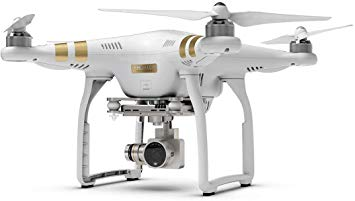
\includegraphics[scale=1]{dji_phantom.jpg}
%
%
%\newpage
%
%\item \textbf{ \Large  Simpler Example:} Quarter Car Suspension Model\\
%
%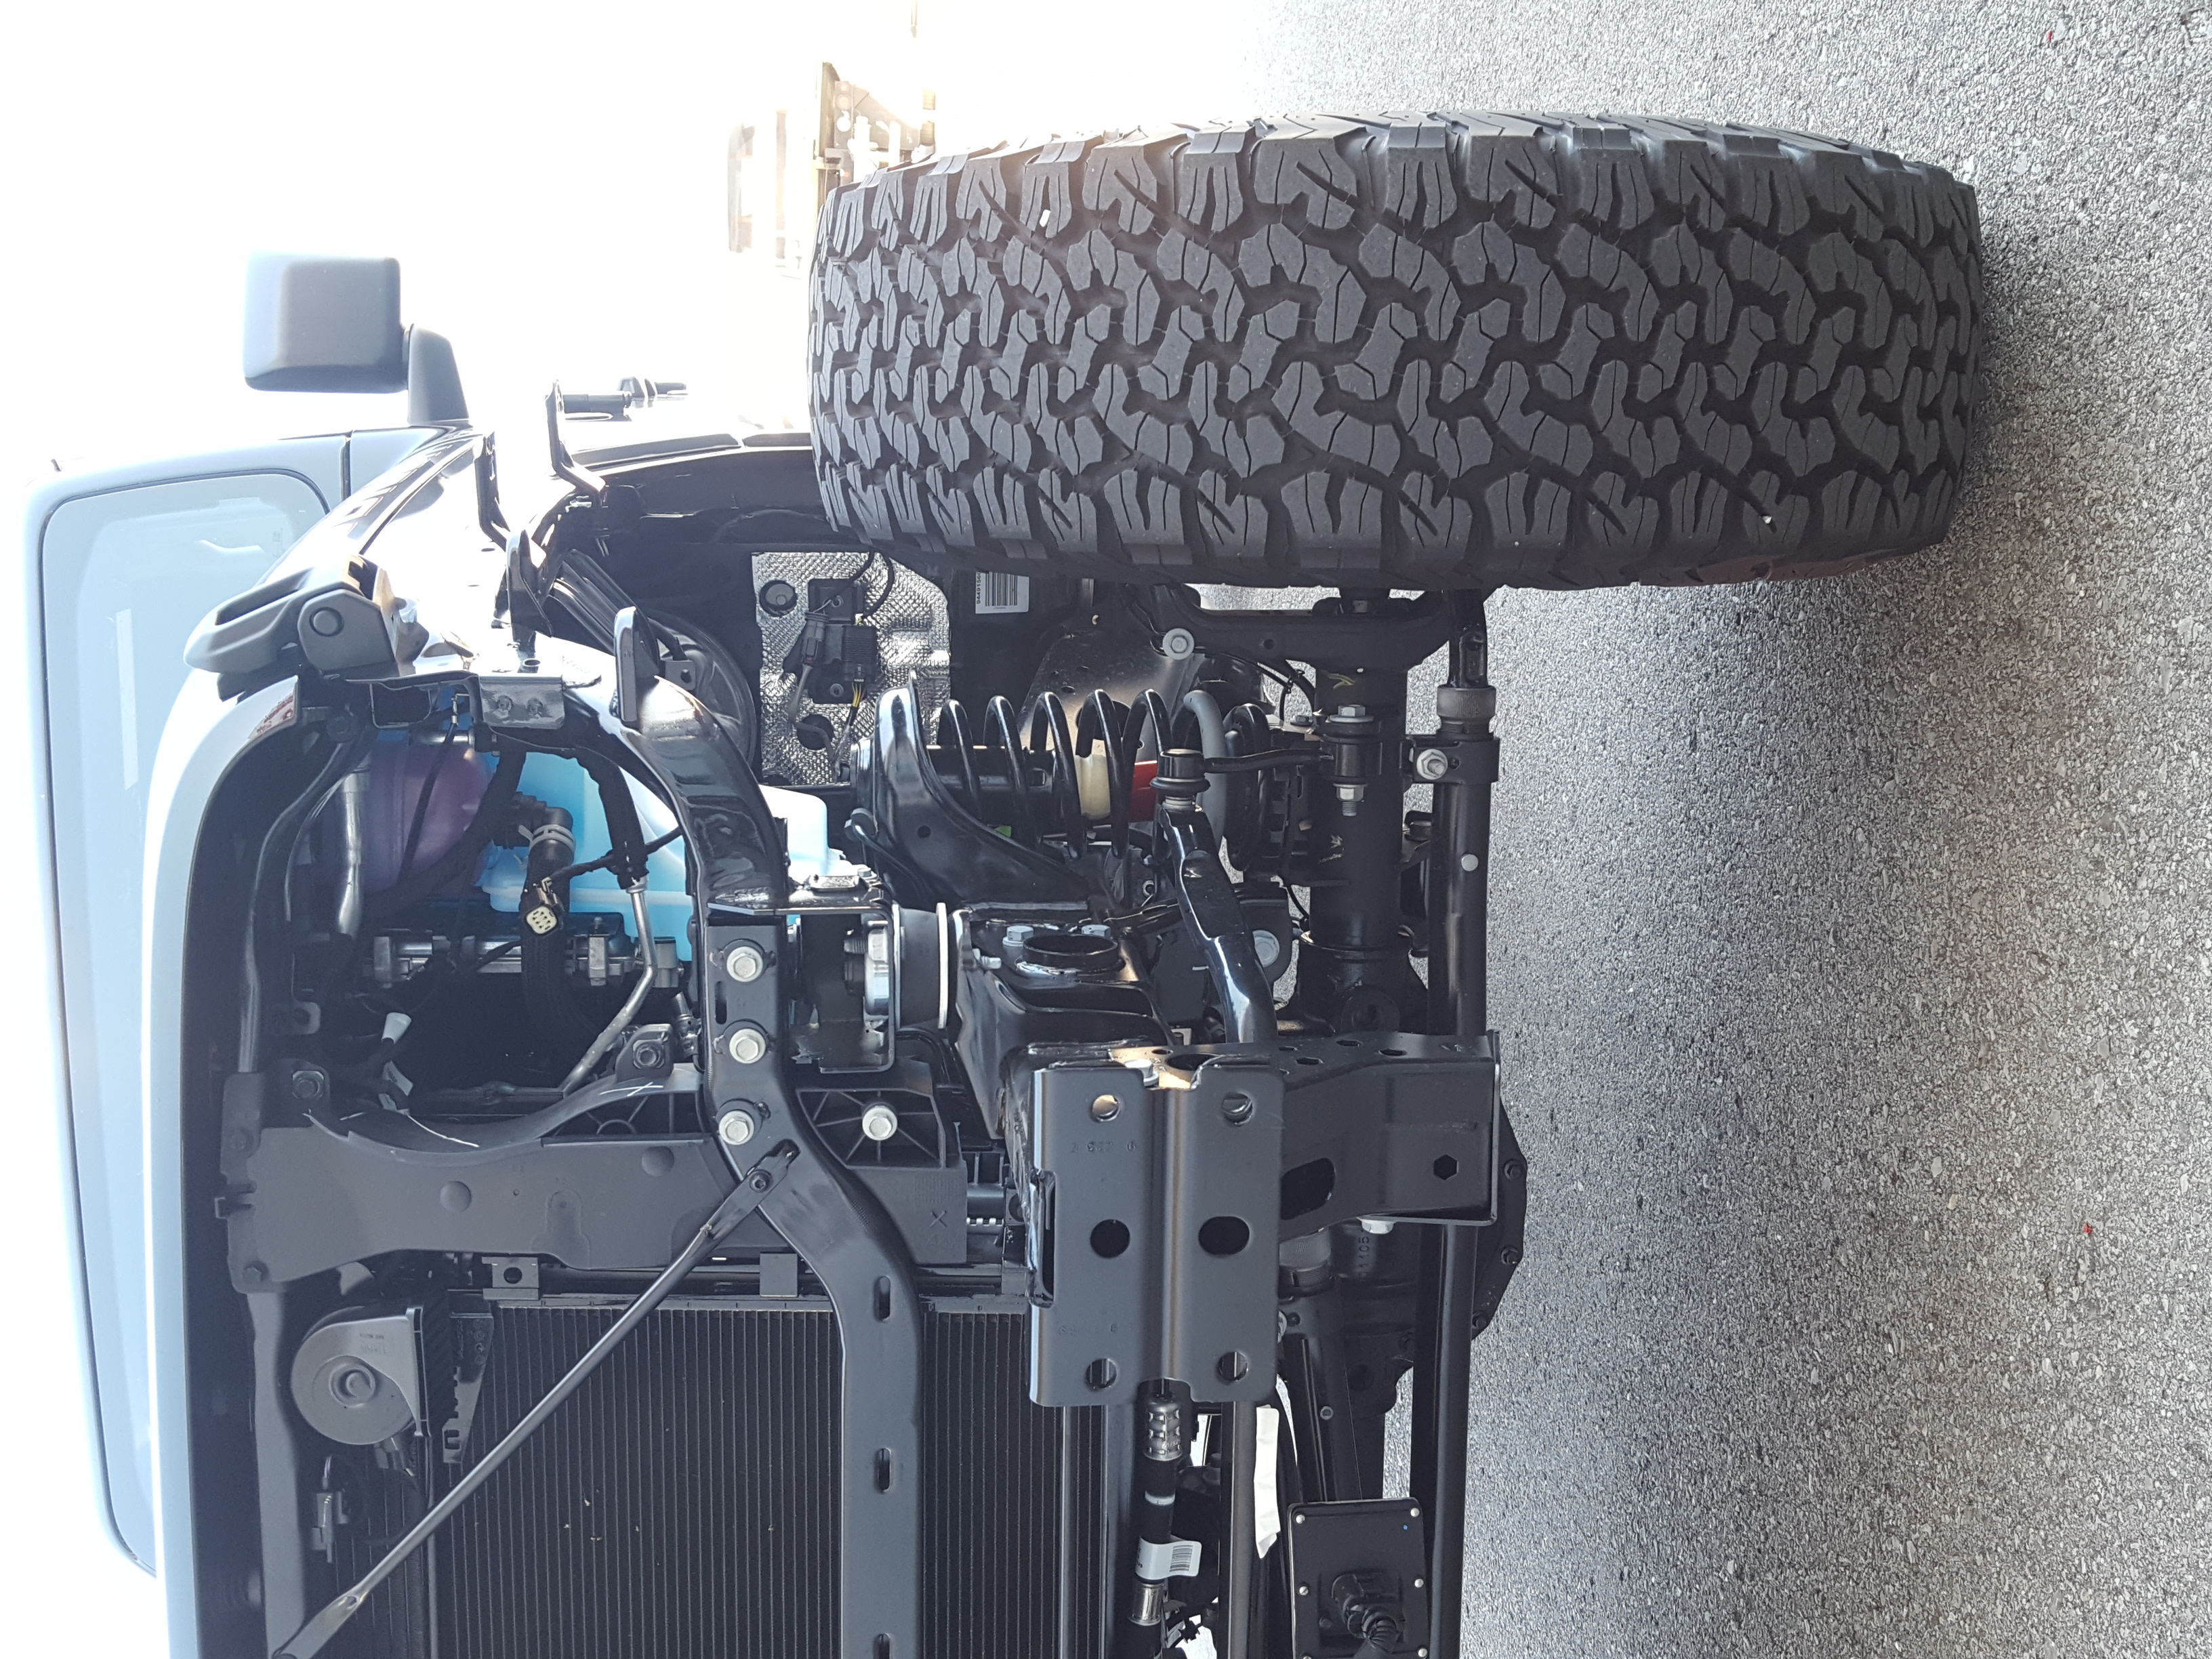
\includegraphics[scale=.1,angle=-90,origin=c]{jeep_01.jpg} 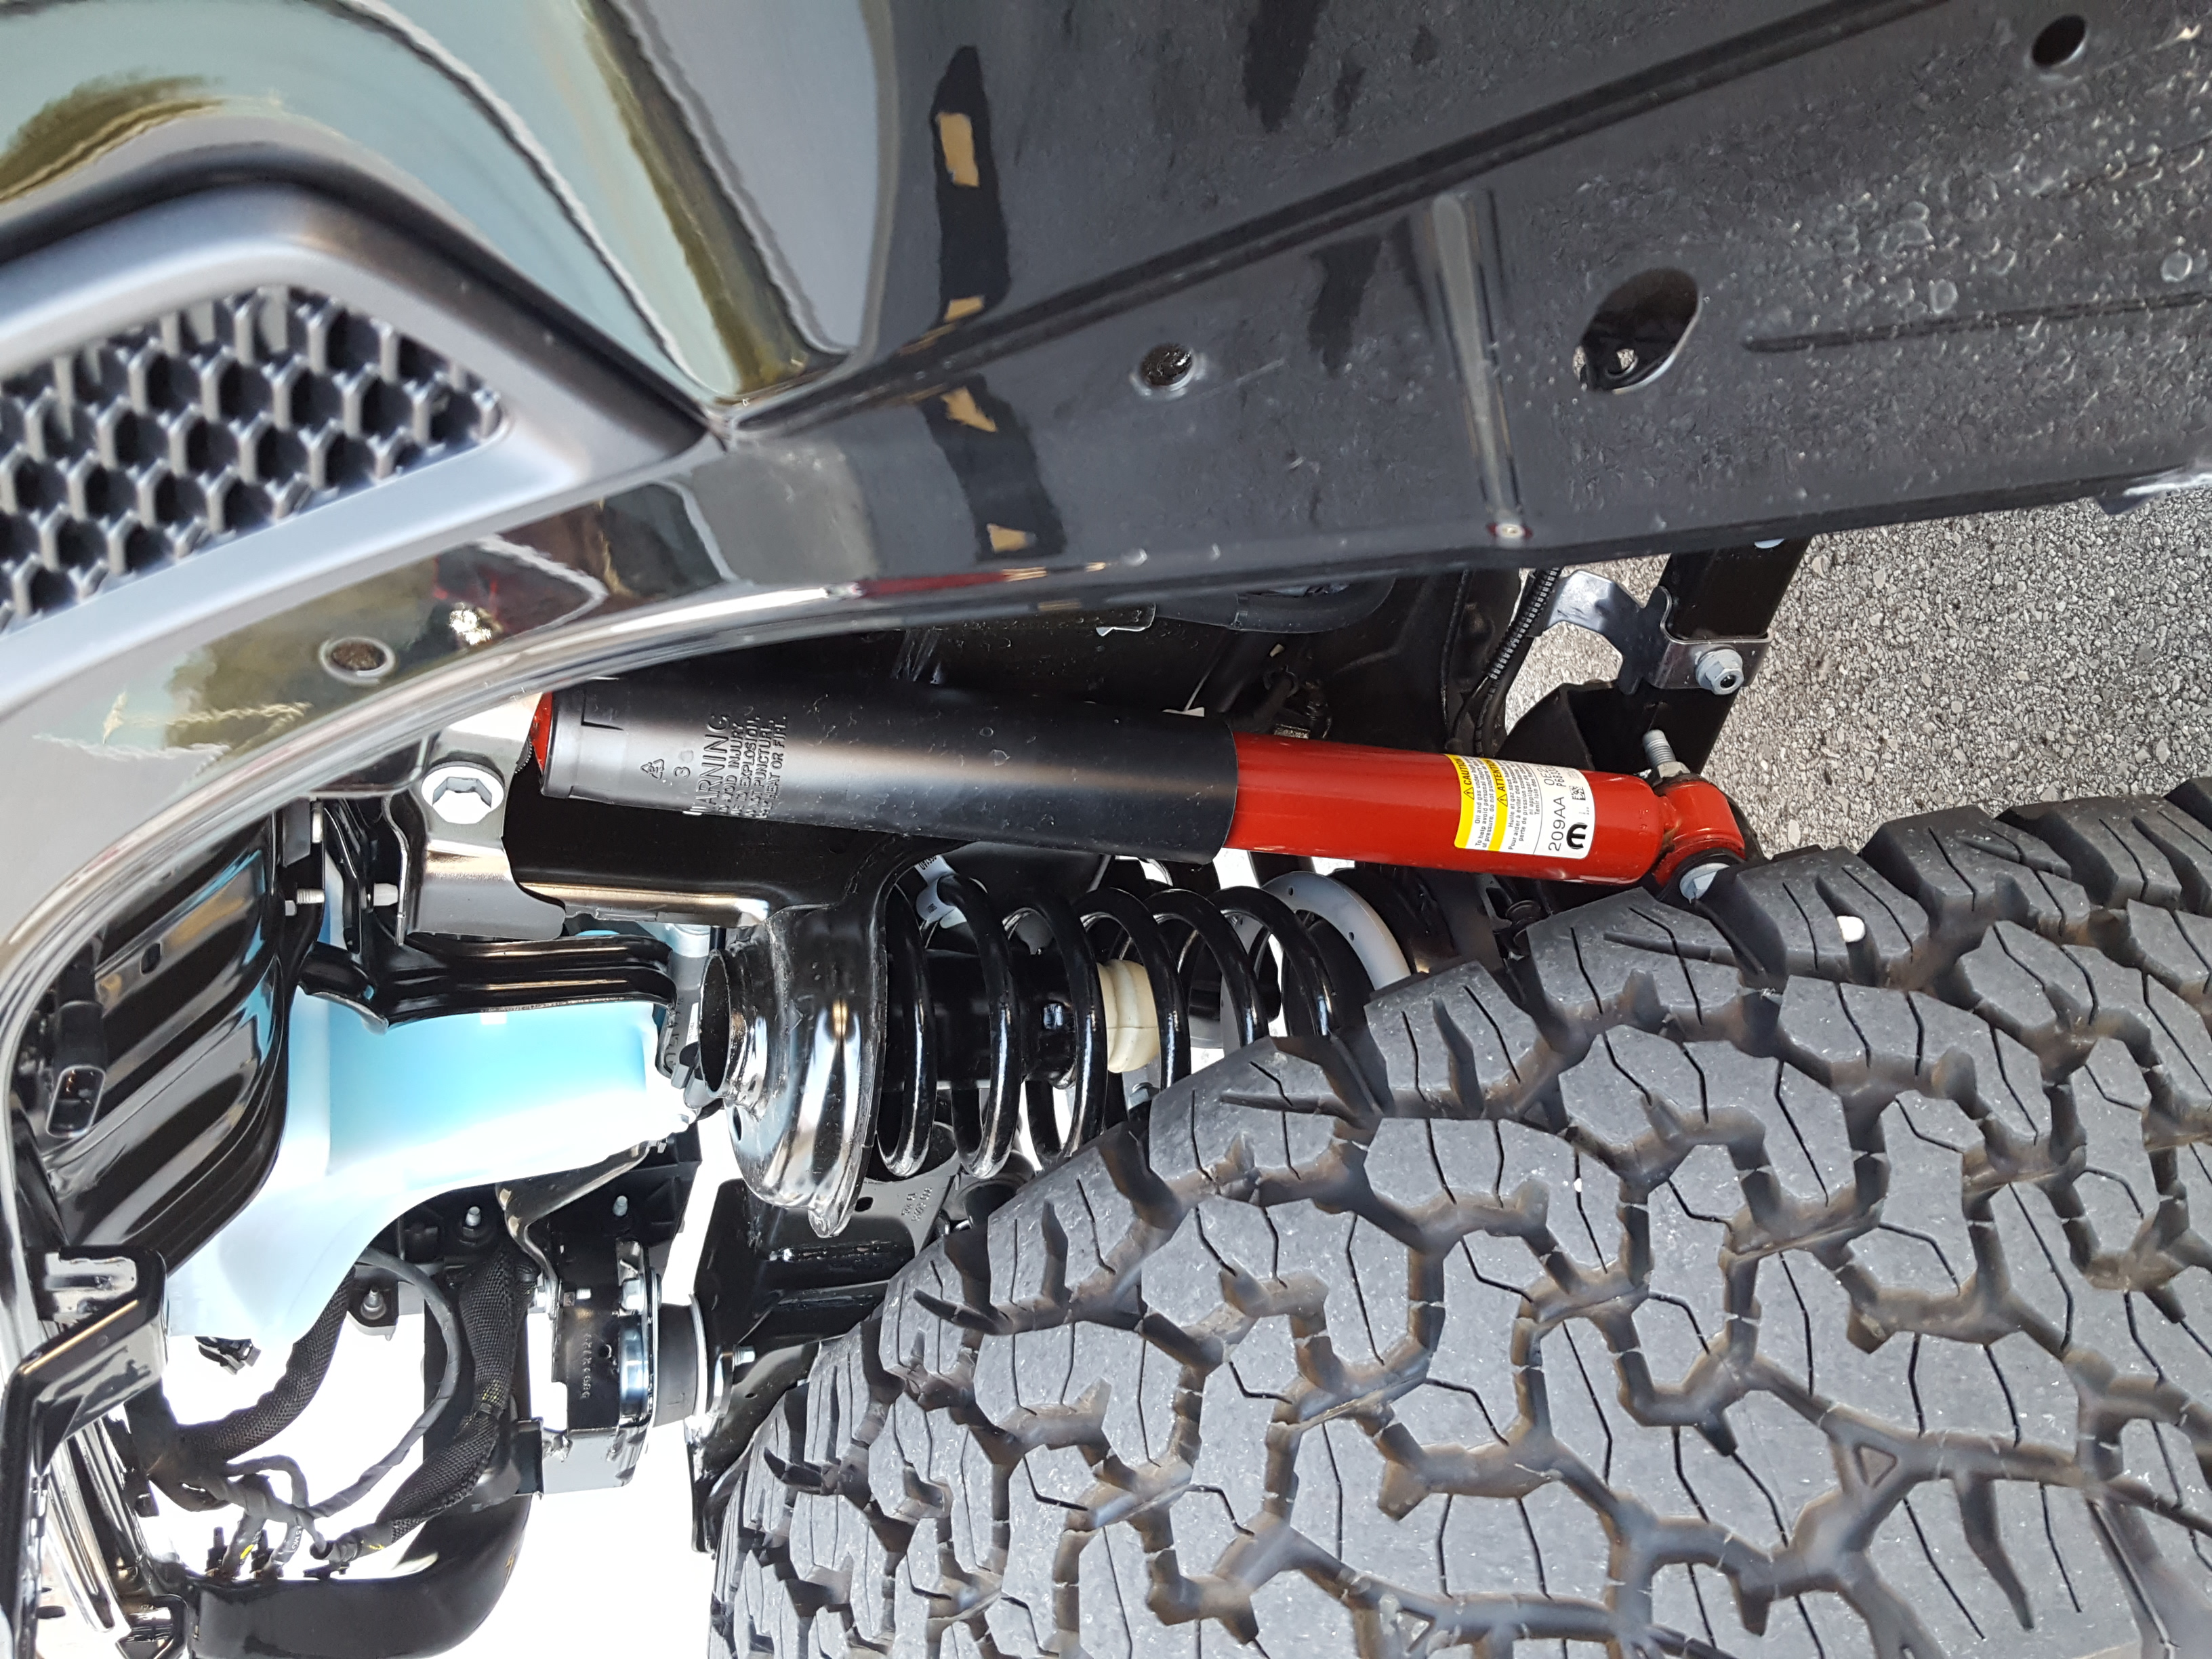
\includegraphics[scale=.1,angle=-90,origin=c]{jeep_02.jpg} \\
%\begin{itemize}
%\item \textbf{ \Large \underline{Problem Statement} -  Derive the \B equations of motion \K using (1) Newton's approach and validate using the (2) Conservation of Energy.}\\
%
%\item \textbf{ \Large \underline{Assumptions} - List the assumptions used in the modeling process.  } 
%
%
%\newpage
%
%\item \textbf{ \Large \underline{Figure(s)} - Draw a \B free body diagram (FBD) \K and/or a sketch of the system. Some problems will require more than one. You need at least one per \B degree of freedom \K.} 
%
%\newpage
%
%\item \textbf{ \Large \underline{Newton's Approach} }\\
%\begin{enumerate}
%\item Draw a Free Body Diagram \vspace{20mm}\\
%\item Determine all \B forces \K acting on the system and their \B directions\K. \vspace{20mm}\\
%\item Write \B Newton's second law \K for the appropriate DOF. \vspace{70mm}\\
%\item Re-write the ODE in the \B standard form \K of a system equation.
%\end{enumerate}
%
%\newpage
%\item \textbf{ \Large \underline{Conservation of Energy Approach} }\\
%\begin{enumerate}
%\item Draw a Free Body Diagram \vspace{20mm}\\
%\item Determine all \B energies \K present in the system and their \B type\K. \vspace{20mm}\\
%\item Write \B Conservation of Energy \K for system. Call this equation 1.\vspace{70mm}\\
%\item Re-write the ODE in the \B standard form \K of a system equation.
%\end{enumerate}
%
%
%\end{itemize}
%
%
%\end{itemize}


	

\end{document}



